\subsection{Distância Total dos Moves}

Somente o peso do custo da distância total dos moves foi alterado para $10$. Os
resultados no planejamento são apresentados na
Figura~\ref{fig:mov_dist_total_10}.

\begin{figure}[H]
  \centering
  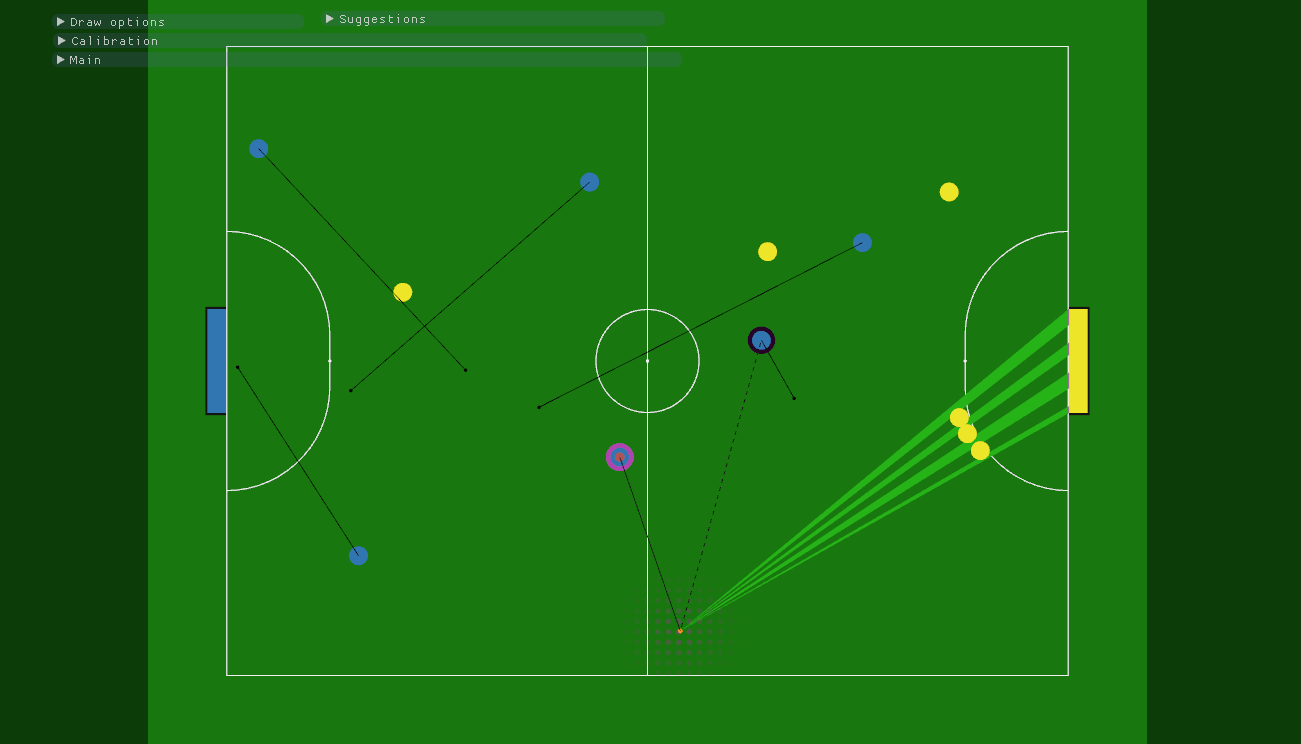
\includegraphics[width= 0.8\linewidth]{result/mov_dist_total_atq_10}
  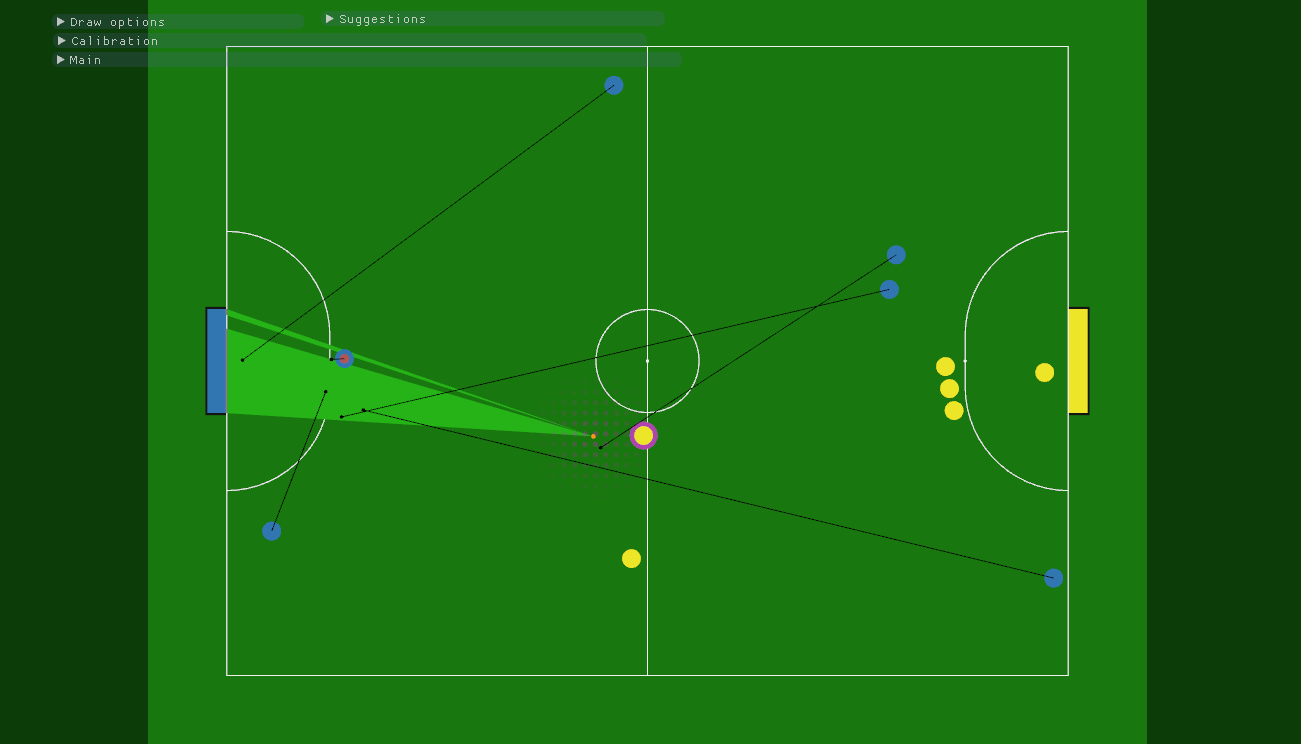
\includegraphics[width= 0.8\linewidth]{result/mov_dist_total_def_10}
  \caption{Planejamento com os parâmetros iniciais e o peso do custo da
  distância total dos moves alterado para $10$.  Ataque (acima) e na defesa (abaixo)}\label{fig:mov_dist_total_10}
\end{figure}

% vim: tw=80 et ts=2 sw=2 sts=2 ft=tex spelllang=pt_br,en
